\documentclass[a4paper, pt14]{article}

\usepackage[utf8]{inputenc}
\usepackage[T1]{fontenc}
\usepackage[slovene]{babel}
\usepackage{lmodern}
%\usepackage{hyperref}
\usepackage{amsmath}
\usepackage{amssymb}
\usepackage{graphicx}


\begin{document}

\title{%
Scheduling-Queues\\
  \large Finančni praktikum}
\author{Špela Bernardič, Ioann Stanković}
\date{10. \ 1. \ 2023}

\maketitle






\section{Navodilo naloge}
Naloga se ukvarja z algoritmi 'Scheduling-Queues', ki uporabljajo podatke napovedane s strojnim učenjem.
Potrebno je napisati simulacijo procesov, ki uporabi napovedane čase trajanja procesov in nato narediti analizo časa čakanja procesov.
Preveriti je potrebno, kako različene porazdelitve trajanja procesov in kvaliteta napovedi vplivata na povprečen čas čakanja v vrsti.
Napovedi časov trajanja procesov se lahko določi z dodajanjem šumov pravim vrednostim, lahko pa se uporabi naučen model.


\section{Opis problema}

S problemom razvrščanja opravil v vrsti se srečamo na različnih področjih. Za opravila nevemo nujno njihove dolžino trajanja, velikokrat pa jo laho ocenimo oziroma napovemo. 
Zato je poleg optimalnosti algoritmov, ki za razvrščanje uporabljajo dejanske čase trajanja opravila, smiselno analizirati tudi, primere, ko se uporabljajo napovedani časi trajanja opravila.
Opazovati je torej treba, povprečen čas čakanja opravila v vrsti. Želimo, da je ta čim krajši.

\section{Potek dela}
\subsection{Algoritmi razvrščanja procesov}

Za reševanje problema razvrščanja procesov v vrsti se uporabljaj različni algoritmi. V nalogi sva uporabila naslednje osnovne algoritme:
\begin{itemize}
  \item FCFS (First Come First Serve) je algoritem, ki izvaja procese po vrstnem redu njihovega prihoda.
  \item SJF (Non-Preemptive Shortest Job First) je algoritem, pri katerem se za naslednjo izvedbo izbere proces z najkrajšim časom trajanja. Ko se določi kateri proces se naj izvede naslednji, se ta izvede do konca. 
  \item PSJF (Preemptive Shortest Job First) je algoritem, pri katerem se proces z najkrajšim časom trajanja začne izvajati prvi. Ob prihodu novega procesa se le ta postavi v čakalno vrsto. Če pa pride proces s krajšim trajanjem od procesa, ki se trenutno izvaja, se trenutni proces ustavi in vrne v vrsto. Začne se izvajati proces s krajšim trajanjem.
  \item SRPT (Shortest remaining processing time) je algoritem podoben PSJF, vendar ta upošteva preostanke trajanj procesov.
\end{itemize}

Poleg osnovnih algoritmov sva napisala še variacje z napovedmi:

\begin{itemize}
  \item SPJF (Non-Preemptive Shortest Predicted Job First) za naslednjo izvedbo izbere proces z najkrajšim \textbf{napovedanim} časom trajanja. Ko se določi kateri proces se naj izvede naslednji, se ta izvede do konca. 
  \item PSPJF (Preemptive Shortest Predicted Job First) proces z najkrajšim \textbf{napovedanim} časom trajanja se začne izvajati prvi. Ob prihodu novega procesa se le ta postavi v čakalno vrsto. Če pride proces s krajšim \textbf{napovedanim} trajanjem od procesa, ki se trenutno izvaja, se trenutni proces ustavi in vrne v vrsto. Začne se izvajati proces s krajšim \textbf{napovedanim} trajanjem.
  \item SPRPT (Shortest Predicted remaining processing time) je algoritem podoben PSJF, vendar ta upošteva preostanek \textbf{napovedanega} trajanj procesov.
\end{itemize}



\subsection{Generiranje podatkov in predikcije}
Za algoritme je bilo potrebno zgenerirat podatke za \v case prihodov opravil, dol\v zine teh opravil, in \v sum na opravilih. Za generiranje podatkov sva uporabila programski jezik R. \v Case prihodov opravil sva zgenerirala z eksponentno porazdelitvijo s parametrom $\lambda = 0.25$, torej $N \sim exp(0.25) $. \v Sum sva dodala z normalno porazdelitvijo, $ Z \sim N(0,\sigma) $ , kjer sva izbrala $\sigma = 0.01$ in nato \v se pogledala kako se grafi obna\v sajo glede na spremembo $\sigma$. Da bi se izognila dolžinam opravil in \v sumu velikosti 0 sva za minimalno dol\v zino opravila vzela $10^{-7}$.

\subsubsection{Generiranje prihodov Beta porazdelitve}
    Za dol\v zine opravil sva v enem primeru uporabila Beta porazdelitev skalirano za 10, torej $X \sim Beta(\alpha, \beta) \times 10 $, z $ E[x] = 5$ in $Var[x] = 1 $ potem $\alpha = \beta = 12$. Zanimalo naju je, tudi \v ce se oblika grafa spremeni ko izberemo majhne dol\v zine opravil, to sva pogledala samo za Beta porazdelitev, tukaj sva vzela $ E[X] = 0.5$, $Var[X] = 0.01 $ in  $Var[Z] = 0.01 $, torej $X \sim Beta(12,12)$.

\subsubsection{Generiranje prihodov Normalne porazdelitve}
  V drugem primeru sva uporabila Normalno porazdelitev $Y \sim |N(5,5)|$, vzela sva absolutno vrednost normalne porazdelitve, da bi se izognila negativnim vrednostim. DEJANSKA VREDNOST UPANJA IN VARIANCE. 



\section{Analiza}
\subsection{Analiza Beta porazdelitve}
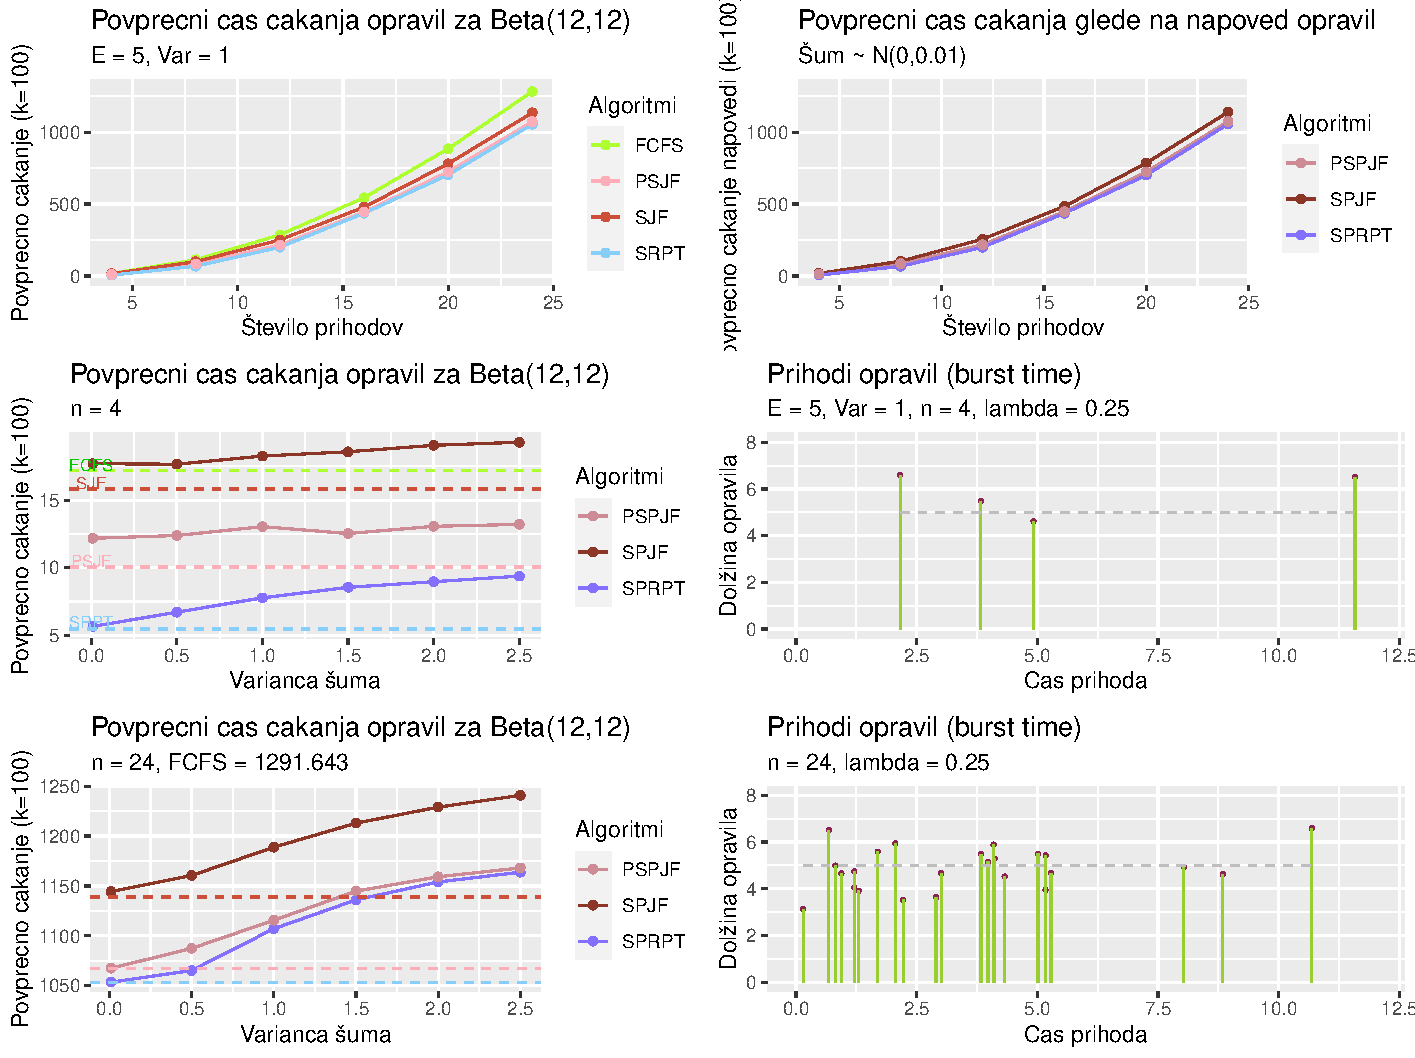
\includegraphics[width=12.1cm,keepaspectratio]{Beta_grafi.pdf}
\\Iz grafov lahko sklepamo, da \v cas povpre\v cnega \v cakanja nara\v s\v ca eksponentno glede na \v stevilo prihodov. Opazimo ve\v cje \v casovno odstopanje za algoritem FCFS, kar nas tudi ne presene\v ca, saj je ta algoritem \v ze za majhno \v stevilo prihodov relativno po\v casen. Mogo\v ce bolj presenetljiv rezultat je, da imamo zelo majhno odstopanje povpre\v cnega \v casa \v cakanja za algoritme z napovedmi, tudi \v ce pove\v camo varianco na 2.5, kar je relativno velik \v sum , ki znatno spremeni za\v cetne podatke. Iz grafov sklepava, da povpre\v cni \v cas \v cakanja nara\v s\v ca linearno s spremembo variance \v suma. Nisva pogledala obna\v sanje algoritmov za ve\v cje variance \v sumov, saj se nam to ni zdelo smiselno.\\
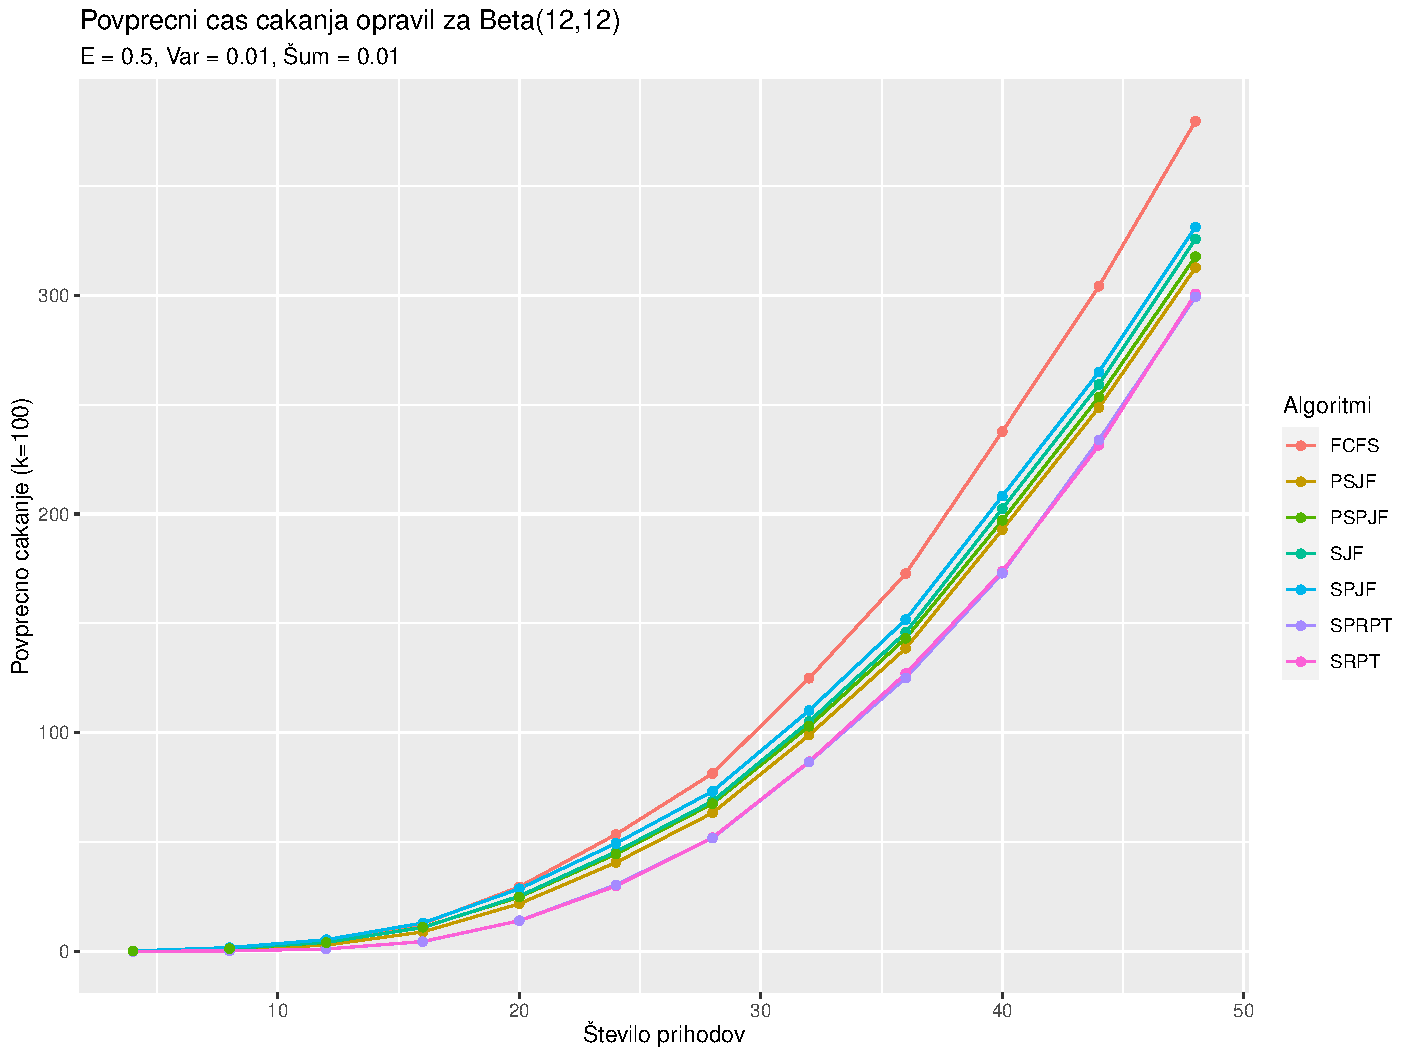
\includegraphics[width=12.1cm,keepaspectratio]{Beta_grafi_majhna.pdf}
\\
Tu so zelo presenetljivi rezultati, ki jih nerazumem

\subsection{Analiza Normalne porazdelitve}

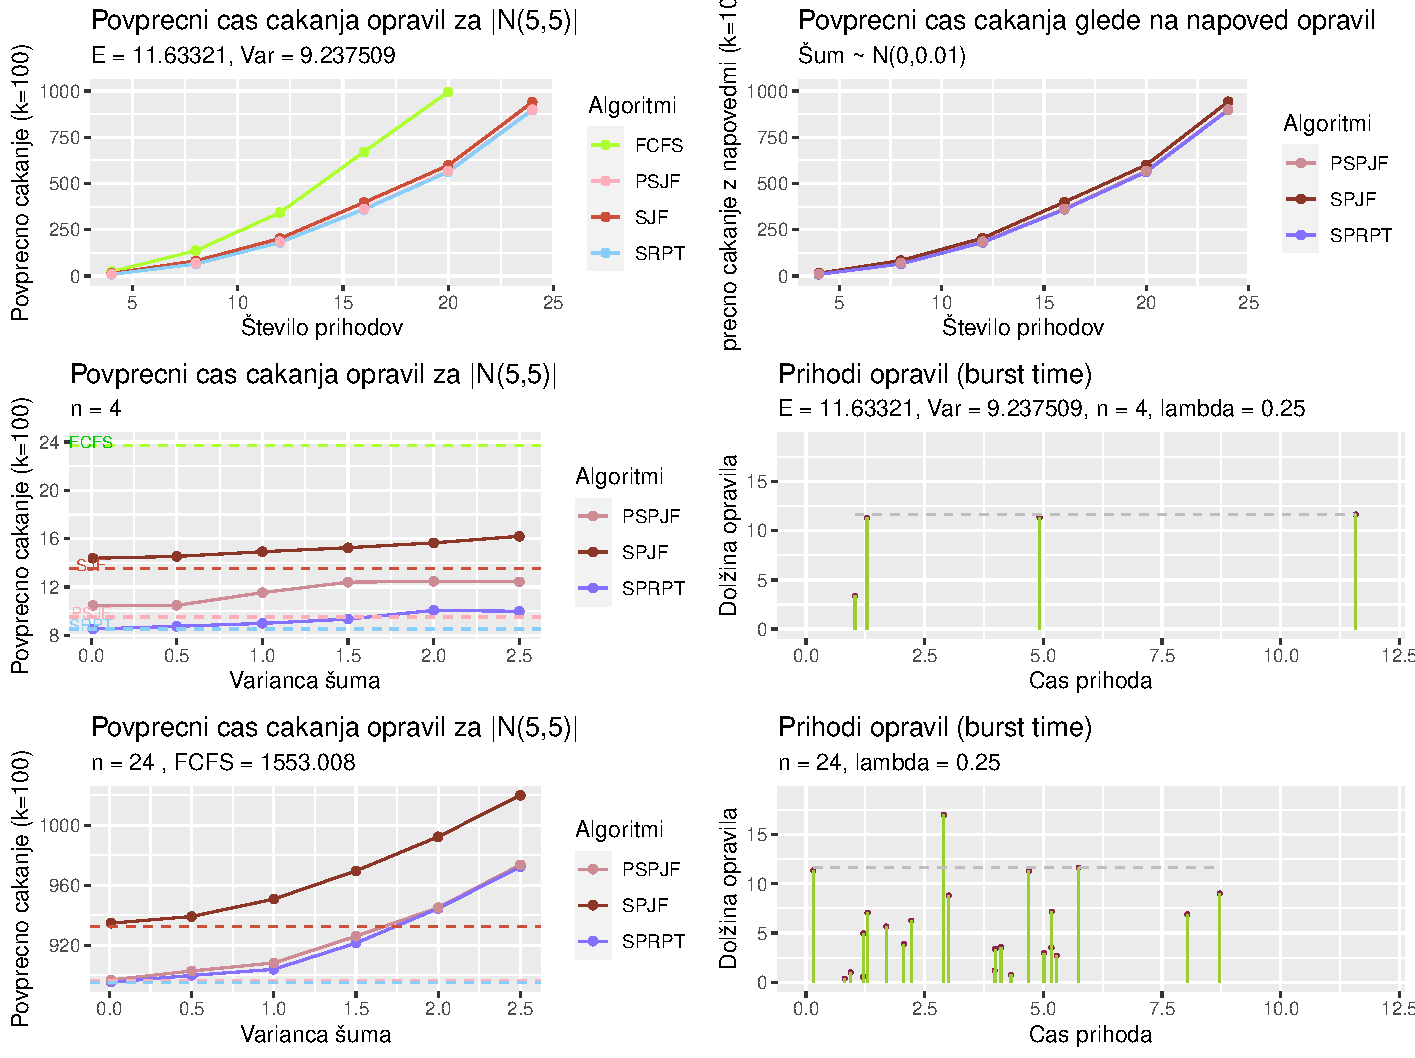
\includegraphics[width=12.1cm,keepaspectratio]{Normalna_grafi.pdf}
\\ Lahko sklepamo podobno kot pri prvi analizi, vendar opazimo \v se ve\v cje odstopanje pri algoritmu FCFS, razlog je da so v tem primeru dol\v zine opravil v povpre\v cju dalj\v se kot pri beta porazdelitvi. 
\end{document}